\documentclass[aspectratio=169]{beamer}

\setbeamersize{text margin left=5mm, text margin right=5mm}

\defbeamertemplate{headline}{my header}{%
\vskip1pt%
\makebox[0pt][l]{\,\insertshortauthor}%
\hspace*{\fill}\insertshorttitle/\insertshortsubtitle\hspace*{\fill}%
\llap{\insertpagenumber/\insertpresentationendpage\,}
}
\setbeamertemplate{headline}[my header]

\let\olditem\item
\renewcommand{\item}{\setlength{\itemsep}{\fill}\olditem}

\usepackage{bm}
\usepackage{graphicx}
\usepackage{caption}
\usepackage{soul}
\usepackage{tkz-euclide}
\usetikzlibrary{calc}
\usepackage[]{algorithm2e}
\usepackage{changepage}
\usepackage{amssymb}
\usepackage{xcolor}
\usepackage{mathtools}
\usepackage{tcolorbox}
\usepackage{tikz}
\usepackage{tikz-3dplot}
\usepackage{tkz-euclide}
\usepackage{circuitikz}
\usepackage{mleftright}
\usetikzlibrary{arrows.meta, decorations.pathreplacing, positioning, shapes.geometric}
\usetikzlibrary{arrows}

\usepackage{pgfplots}
\usetikzlibrary{plotmarks}
\pgfplotsset{width=7cm,compat=1.8}
\pgfplotsset{compat=1.17}

\usetikzlibrary{positioning}
% \usepackage[math]{cellspace}
% \cellspacetoplimit 4pt
% \cellspacebottomlimit 4pt
%\usetikzlibrary{arrows.meta}
% sqare of half axes
\newcommand{\asa}{3}
\newcommand{\bsa}{1}
\newcommand{\csa}{0.25}
% view angle
\tdplotsetmaincoords{70}{135}


%% Fonts
\usefonttheme{professionalfonts}
\usefonttheme{serif}

\DeclareCaptionLabelFormat{blank}{}
\captionsetup[figure]{labelformat=blank}

%% Math definitions
\def\mf{\ensuremath\mathbf}
\def\mb{\ensuremath\mathbb}
\def\mc{\ensuremath\mathcal}
\def\lp{\ensuremath\left(}
\def\rp{\ensuremath\right)}
\def\lv{\ensuremath\left\lvert}
\def\rv{\ensuremath\right\rvert}
\def\lV{\ensuremath\left\lVert}
\def\rV{\ensuremath\right\rVert}
\def\lc{\ensuremath\left\{}
\def\rc{\ensuremath\right\}}
\def\ls{\ensuremath\left[}
\def\rs{\ensuremath\right]}
\def\bmx{\ensuremath\begin{bmatrix*}[r]}
\def\emx{\ensuremath\end{bmatrix*}}
\def\bmxc{\ensuremath\begin{bmatrix*}[c]}
\def\t{\lp t\rp}
\def\k{\ls k\rs}

\newcommand{\demoex}[2]{\onslide<#1->\begin{color}{black!60} #2 \end{color}}
\newcommand{\demoexc}[3]{\onslide<#1->\begin{color}{#2} #3 \end{color}}
\newcommand{\anim}[3]{\onslide<#1->{\begin{color}{#2!60} #3 \end{color}}}
\newcommand{\ct}[1]{\lp #1\rp}
\newcommand{\dt}[1]{\ls #1\rs}
\newcommand{\cols}[2]{\begin{columns}[#1] #2 \end{columns}}
\newcommand{\col}[2]{\begin{column}{#1} #2 \end{column}}

%% Mycolors
\definecolor{myred}{RGB}{192,0,0}
\definecolor{mygray}{RGB}{100,100,100}

%% Custom beamer color
\setbeamercolor{title}{fg=myred}
\setbeamercolor{subtitle}{fg=myred}
\setbeamerfont{title}{series=\bfseries}
% \setbeamercolor{frametitle}{bg=myred, fg=white}
\setbeamercolor{frametitle}{bg=mygray!10!, fg=myred}
\setbeamerfont{frametitle}{series=\bfseries}
\setbeamercolor{item}{fg=mygray}
\setbeamercolor{title in head/foot}{fg=myred}

% Move header to footer
\setbeamertemplate{headline}{}
\setbeamertemplate{footline}{
  \begin{beamercolorbox}[wd=\paperwidth,ht=2.25ex,dp=1ex,center]{footline}
    \inserttitle\hfill\insertauthor\hfill\insertdate\hfill\insertframenumber{}
  \end{beamercolorbox}
}

\pgfplotsset{
colormap={whitered}{color(0cm)=(white); color(1cm)=(orange!75!red)}
}


\title{Applied Linear Algebra for Data}

% A subtitle is optional and this may be deleted
\subtitle{Linear Programming}

\author{Sivakumar Balasubramanian}
% - Give the names in the same order as the appear in the paper.
% - Use the \inst{?} command only if the authors have different
%   affiliation.

\institute[Christian Medical College] % (optional, but mostly needed)
{
  \inst{}%
  Department of Bioengineering\\
  Christian Medical College, Bagayam\\
  Vellore 632002
}
% - Use the \inst command only if there are several affiliations.
% - Keep it simple, no one is interested in your street address.

\date{}
% - Either use conference name or its abbreviation.
% - Not really informative to the audience, more for people (including
%   yourself) who are reading the slides online

\subject{Lecture notes on ALADA}
% This is only inserted into the PDF information catalog. Can be left
% out. 

% If you have a file called "university-logo-filename.xxx", where xxx
% is a graphic format that can be processed by latex or pdflatex,
% resp., then you can add a logo as follows:

% \pgfdeclareimage[height=0.5cm]{university-logo}{university-logo-filename}
% \logo{\pgfuseimage{university-logo}}

% Delete this, if you do not want the table of contents to pop up at
% the beginning of each subsection:
\AtBeginSubsection[]
{
  \begin{frame}<beamer>{Outline}
    \tableofcontents[currentsection,currentsubsection]
  \end{frame}
}

% Let's get started
\begin{document}

\pgfplotsset{
  compat=1.8,
  colormap={whitered}{color(0cm)=(white); color(1cm)=(orange!75!red)}
}

\begin{frame}
  \titlepage
\end{frame}

% \begin{frame}[t]{References}
% \begin{itemize}
%     \item G Strang, Linear Algebra: Chapters .
% \end{itemize} 
% \end{frame}


% \begin{frame}[t]{Linear Programming}
%   Linear programming problems are a class of optimization problems where $f(\mf{x})$ is linear and $h(\mf{x})$, $g(\mf{x})$ are affine functions.

%   There are different ways in which \textit{linear programming} problems are formulated. The standard (equality) form of the linear programming problem,
%   \[ \begin{split}
%         \text{minimize} & \quad \mf{c}^\top \mf{x} \\
%         \text{subject to} & \quad \mf{A}\mf{x} = \mf{b} \\
%         & \quad \mf{x} \geq \mf{0}
%      \end{split} \]
%   where, $\mf{x} \in \mathbb{R}^n$, $\mf{A} \in \mathbb{R}^{m \times n}$, and $m < n$.

%   Note that without the constraints the function $\mf{c}^\top\mf{x}$ does not have a minimum. \textcolor{blue}{Why?}

%   Several variation of the above problem are possible, but all of them can be modified to the standard form by suitable modification of $\mf{A}$, $\mf{b}$, $\mf{c}$, and by including additional \textit{dummy} variables.
% \end{frame}


% \begin{frame}[t]{Linear Programming}
%   \textbf{Example.} A company can produces four products $P_1$, $P_2$, $P_3$, and $P_4$. The production of these products requires three resources: raw material 1 $R_1$, raw material $R_2$  and labor $R_3$. The following table shows the amount of each resource required for fabricating each product ($a_{ij}$ the amount of resource $j$ required to produce product $i$). The amount of each of three resources available for production is limited $\lc b_i \rc_{i=1}^3$, and each product has a profit margin $\lc c_i \rc_{i=1}^4$. How much of each product $\lc x_i \rc_{i=1}^4$ should the company produce using the available resources to maximize its proft.

%   \begin{table}
%     \centering
%     \begin{tabular}{c|cccc}
%       & $P_1$ & $P_2$ & $P_3$ & $P_4$ \\
%       \hline
%       $R_1$ & 1 & 2 & 2 & 1 \\
%       $R_2$ & 2 & 1 & 1 & 2 \\
%       $R_3$ & 1 & 1 & 2 & 1 \\
%       \hline
%       Profit & 3 & 2 & 5 & 4
%     \end{tabular}
%   \end{table}
%  Resource limitations for the three resources are $\lc 15, 20, 15 \rc$.
% \end{frame}


% \begin{frame}[t]{Linear Programming}
%   \[ 
%     \begin{split}
%       \text{minimize} & \quad -\ct{3x_1 + 2x_2 + 5x_3 + 4x_4} \\
%       \text{subject to} & \quad 1x_1 + 2x_2 + 2x_3 + 1x_4 \leq 15 \\
%       & \quad 2x_1 + 1x_2 + 1x_3 + 2x_4 \leq 20 \\
%       & \quad 1x_1 + 1x_2 + 2x_3 + 1x_4 \leq 15 \\
%       & \quad x_1, x_2, x_3, x_4 \geq 0
%     \end{split}
%   \]
%   Here, $\mf{c} = \bmx -3 & -2 & -5 & -4\emx^\top$, $\mf{A} = \bmx 1 & 2  & 2 & 1 \\ 2 & 1 & 1 & 2 \\ 1 & 1 & 2 & 1 \emx$, $\mf{b} = \bmx 15 \\ 20 \\ 15\emx$, and $\mf{x} = \bmx x_1 \\ x_2 \\ x_3 \\ x_4\emx$.
% \end{frame}


% \begin{frame}[t]{Linear Programming}
%   The above problem is not in the standard form. We can convert this into the standard from by adding three dummy variables $x_5, x_6,$ and  $x_7$, such that we convert the inequality $\mf{A}\mf{x} \leq \mf{b}$ as the following,
%   \[ 
%     \begin{split}
%       \text{minimize} & \quad -\ct{3x_1 + 2x_2 + 5x_3 + 4x_4} \\
%       \text{subject to} & \quad 1x_1 + 2x_2 + 2x_3 + 1x_4 + x_5 = 15 \\
%       & \quad 2x_1 + 1x_2 + 1x_3 + 2x_4 + x_6 = 20 \\
%       & \quad 1x_1 + 1x_2 + 2x_3 + 1x_4 + x_7 = 15 \\
%       & \quad x_1, x_2, x_3, x_4, x_5, x_6, x_7 \geq 0
%     \end{split}
%   \]
%   Here, $\tilde{\mf{c}} = \bmx \mf{c} \\ \mf{0} \emx$, $\tilde{\mf{A}} = \bmx \mf{A} & \mf{I} \emx$, and $\tilde{\mf{x}} = \bmxc x_1 \\ \vdots \\ x_7\emx$.
% \end{frame}


% \begin{frame}[t]{Linear Programming}
%   \begin{columns}
%     \column{0.5\textwidth}
%     \[
%       \begin{split}
%         \text{minimize} & \quad -x_1 - 2x_2 \\
%         \text{subject to} & \quad x_1 + x_2 \leq 5 \\ 
%         & \quad x_1, x_2 \geq 0
%       \end{split}
%     \]
%     This LP is in the non-standard form. This can be converted to the standard form by adding a slack variable $x_3$.
%     \vspace{0.2cm}
    
%     A graphical visualization of this LP is shown on the right.

%     \column{0.42\textwidth}
%     \begin{figure}
%       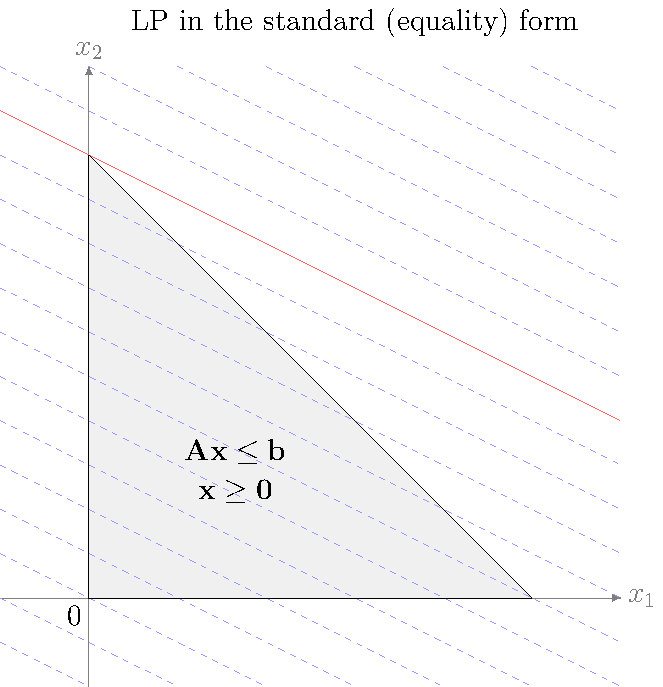
\includegraphics[width=\textwidth]{figs/lpnonstand.pdf}
%     \end{figure}
%   \end{columns}
% \end{frame}


% \begin{frame}[t]{Linear Programming}
%   \begin{columns}
%     \column{0.5\textwidth}
%     \[
%       \begin{split}
%         \text{minimize} & \quad -x_1 - 2x_2 \\
%         \text{subject to} & \quad x_1 + x_2 + x_3 = 5 \\ 
%         & \quad x_1, x_2, x_3 \geq 0
%       \end{split}
%     \]
%     This LP is in the standard form, but has a higher dimension than the original problem. The search now is on a simplex, as shown in the figure on the right.

%     \column{0.42\textwidth}
%     \begin{figure}
%       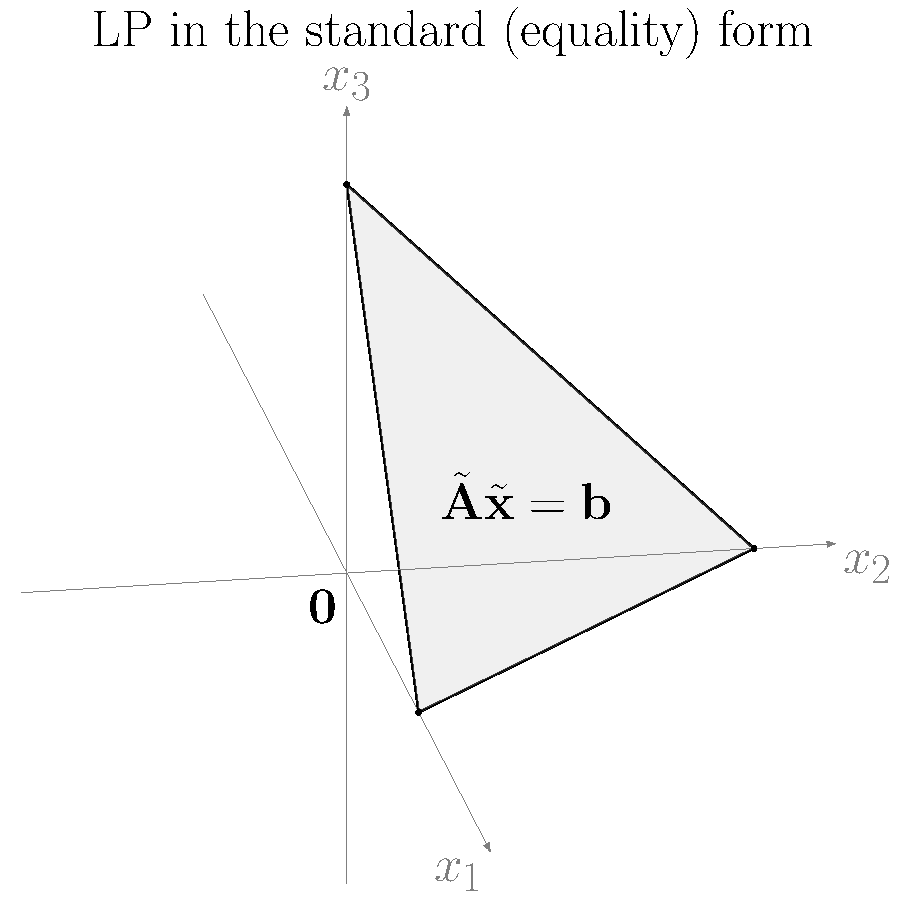
\includegraphics[width=\textwidth]{figs/lpstand.pdf}
%     \end{figure}
%   \end{columns}
% \end{frame}


\begin{frame}[t]{Linear Programming: Examples}
  \textbf{Example.} A prosthetics and orthotics department produces three types of assistive devices -- Ankle Foot Orthosis (AFO), Knee Brace (KB), and Wrist Splint (WB). The production of these products requires three types of resources: metal, plastics and labor. The following table shows the amount of each resource required for fabricating each product . The amount of each of the three resources available for production is limited 20 units of metal, 30 units of plastic nad 25 units of labor. How much of each product $\lc x_i \rc_{i=1}^3$ should the company produce using the available resources to maximize its productivity. Fractional amount of products are allowed.
  \begin{table}[]
    \begin{tabular}{|l|l|l|l|}
    \hline
    \multicolumn{1}{|c|}{\textbf{Item}} & \multicolumn{1}{c|}{\textbf{Metal}} & \multicolumn{1}{c|}{\textbf{Plastic}} & \multicolumn{1}{c|}{\textbf{Labor}} \\ \hline
    Ankle Foot Orthosis (AFO) & 2 & 4 & 4 \\ \hline
    Knee Brace (KB) & 4 & 3 & 5 \\ \hline
    Wrist Splint (WS) & 1 & 2 & 2 \\ \hline
    \end{tabular}
    \end{table}
\end{frame}


\begin{frame}[t]{Linear Programming: Examples}
  \textbf{Example.} Five patients with a highly infectious drug resistant infection are admitted to a hospital. The hospital has a set of 4 drugs that can be used to treat the infection, but the amount of benefit/harm vaused by each of these drugs is different for each patient. given by the benfit matrix $\mf{B} \in \mb{R}^{5 \times 4}$, where the $b_{ij}$ terms indicates the amount of benefit (or harm) caused by drug $j$ to patient $i$ (+ve $\implies $beneft and -ve $\implies$ harm). The hospital has a limited supply of each drug, given by the vector $\bm{\mu} \in \mb{R}^4$. The hospital wants to maximize the total benefit to the patients by choosing the right combination of drugs for each patient. Formulate this as a linear programming problem.
\end{frame}


\end{document}